% Anhang content
%
\chapter{Configuration File} \label{app:txtConfigFile}%
%
A sample configuration file saved on the SD card looks as can be seen below
\begin{lstlisting}

;========================================================================================
[BaudRateConfiguration]
;
;
; BAUD_RATES_WIRELESS_CONN
; Configuration of baud rates on wireless side from 0 to 3.
; Regarding the supported baud rates see implementation of hwBufIfConfigureBaudRate in hwBufferInterface.cpp
BAUD_RATES_WIRELESS_CONN = 57600, 38400, 57600, 57600
;
;
; BAUD_RATES_DEVICE_CONN
; Configuration of baud rates on wireless side from 0 to 3.
; Regarding the supported baud rates see implementation of hwBufIfConfigureBaudRate in hwBufferInterface.cpp
BAUD_RATES_DEVICE_CONN = 57600, 57600, 38400, 38400
;
;
;========================================================================================
[ConnectionConfiguration]
;
;
; PRIO_WIRELESS_CONN_DEV_X
; Priority of the different wireless connections from the viewpoint of a single device.
; 0: Wireless connection is not used; 1: Highes priority; 2: Second priority, ..
PRIO_WIRELESS_CONN_DEV_0 = 1, 0, 0, 0
PRIO_WIRELESS_CONN_DEV_1 = 0, 1, 0, 0
PRIO_WIRELESS_CONN_DEV_2 = 0, 0, 1, 0
PRIO_WIRELESS_CONN_DEV_3 = 0, 0, 0, 1
;
;
; SEND_CNT_WIRELESS_CONN_DEV_X
; Number of times a package should be tried to be sent over a single wireless connection.
SEND_CNT_WIRELESS_CONN_DEV_0 = 1, 0, 0, 0
SEND_CNT_WIRELESS_CONN_DEV_1 = 0, 1, 0, 0
SEND_CNT_WIRELESS_CONN_DEV_2 = 0, 0, 1, 0
SEND_CNT_WIRELESS_CONN_DEV_3 = 0, 0, 0, 1
;
;
;========================================================================================
[TransmissionConfiguration]
;
;
; RESEND_DELAY_WIRELESS_CONN_DEV_X
; Time in ms that should be waited until a package is sent again when no acknowledge is 
; received per device and wireless connection.
RESEND_DELAY_WIRELESS_CONN_DEV_0 = 3, 3, 3, 3
RESEND_DELAY_WIRELESS_CONN_DEV_1 = 3, 3, 3, 3
RESEND_DELAY_WIRELESS_CONN_DEV_2 = 255, 255, 255, 255
RESEND_DELAY_WIRELESS_CONN_DEV_3 = 255, 255, 255, 255
;
;
; MAX_THROUGHPUT_WIRELESS_CONN
; Maximal throughput per wireless connection (0 to 3) in bytes/s.
MAX_THROUGHPUT_WIRELESS_CONN	 = 10000, 10000, 10000, 10000
;
;
; USUAL_PACKET_SIZE_DEVICE_CONN
; Usual packet size per device in bytes if known or 0 if unknown.
USUAL_PACKET_SIZE_DEVICE_CONN	= 25, 25, 1, 1
;
;
; PACKAGE_GEN_MAX_TIMEOUT
; Maximal time in ms that is waited until packet size is reached. If timeout is reached, 
; the packet will be sent anyway, independent of the amount of the available data.
PACKAGE_GEN_MAX_TIMEOUT	= 2, 2, 20, 20
;
;
; DELAY_DISMISS_OLD_PACK_PER_DEV
DELAY_DISMISS_OLD_PACK_PER_DEV	= 10000, 10000, 10000, 10000
;
;
; SEND_ACK_PER_WIRELESS_CONN
; To be able to configure on which wireless connections acknowledges should be sent if a 
; data package has been received. Set to 0 if no acknowledge should be sent, 1 if yes.
SEND_ACK_PER_WIRELESS_CONN	= 0, 1, 0, 0
;
;
; USE_CTS_PER_WIRELESS_CONN
; To be able to configure on which wireless connections CTS for hardware flow control 
; should be used. Set to 0 if it shouldn't be used, 1 if yes.
; If enabled, data transmission is stopped CTS input is high and continued if low.
USE_CTS_PER_WIRELESS_CONN	= 0, 0, 0, 0
;
;
;========================================================================================
[SoftwareConfiguration]
;
;
; TEST_HW_LOOPBACK_ONLY
; Set to 0 for normal operation, 1 in order to enable loopback on all serial interfaces 
; in order to test the hardware.
TEST_HW_LOOPBACK_ONLY	= 0
;
; GENERATE_DEBUG_OUTPUT
; Set to 0 for normal operation, 1 in order to print out debug infos 
; (might be less performant).
GENERATE_DEBUG_OUTPUT	= 1;
;
; SPI_HANDLER_TASK_INTERVAL
; Interval in [ms] of corresponding task which he will be called. 0 would be no delay - 
; so to run as fast as possible.
SPI_HANDLER_TASK_INTERVAL	= 5;
;
; PACKAGE_GENERATOR_TASK_INTERVAL
; Interval in [ms] of corresponding task which he will be called. 0 would be no delay - 
; so to run as fast as possible.
PACKAGE_GENERATOR_TASK_INTERVAL	= 5;
;
; NETWORK_HANDLER_TASK_INTERVAL
; Interval in [ms] of corresponding task which he will be called. 0 would be no delay - 
; so to run as fast as possible.
NETWORK_HANDLER_TASK_INTERVAL	= 5;
;
; TOGGLE_GREEN_LED_INTERVAL
; Interval in [ms] in which the LED will be turned off or on -> frequency = 2x interval
TOGGLE_GREEN_LED_INTERVAL	= 500
;
; THROUGHPUT_PRINTOUT_TASK_INTERVAL
; Interval in [s] in which the throughput information will be printed out
THROUGHPUT_PRINTOUT_TASK_INTERVAL = 5
;
; SHELL_TASK_INTERVAL
; Interval in [ms] in which the shell task is called to refresh the shell 
; (which prints debug information and reads user inputs)
SHELL_TASK_INTERVAL		= 10
\end{lstlisting}
%
\section{Unterkapitel im Anhang} \label{refSectionAnhang}%
%
\blindtext%
%
\subsection{Tieferes Kapitel}%
%
\subsubsection{Noch tieferes Kapitel}%
%
\blindtext%
%
%
%
\chapter{Task Description} \label{app:Aufgabenstellung}
The full task description for this project can be found below.
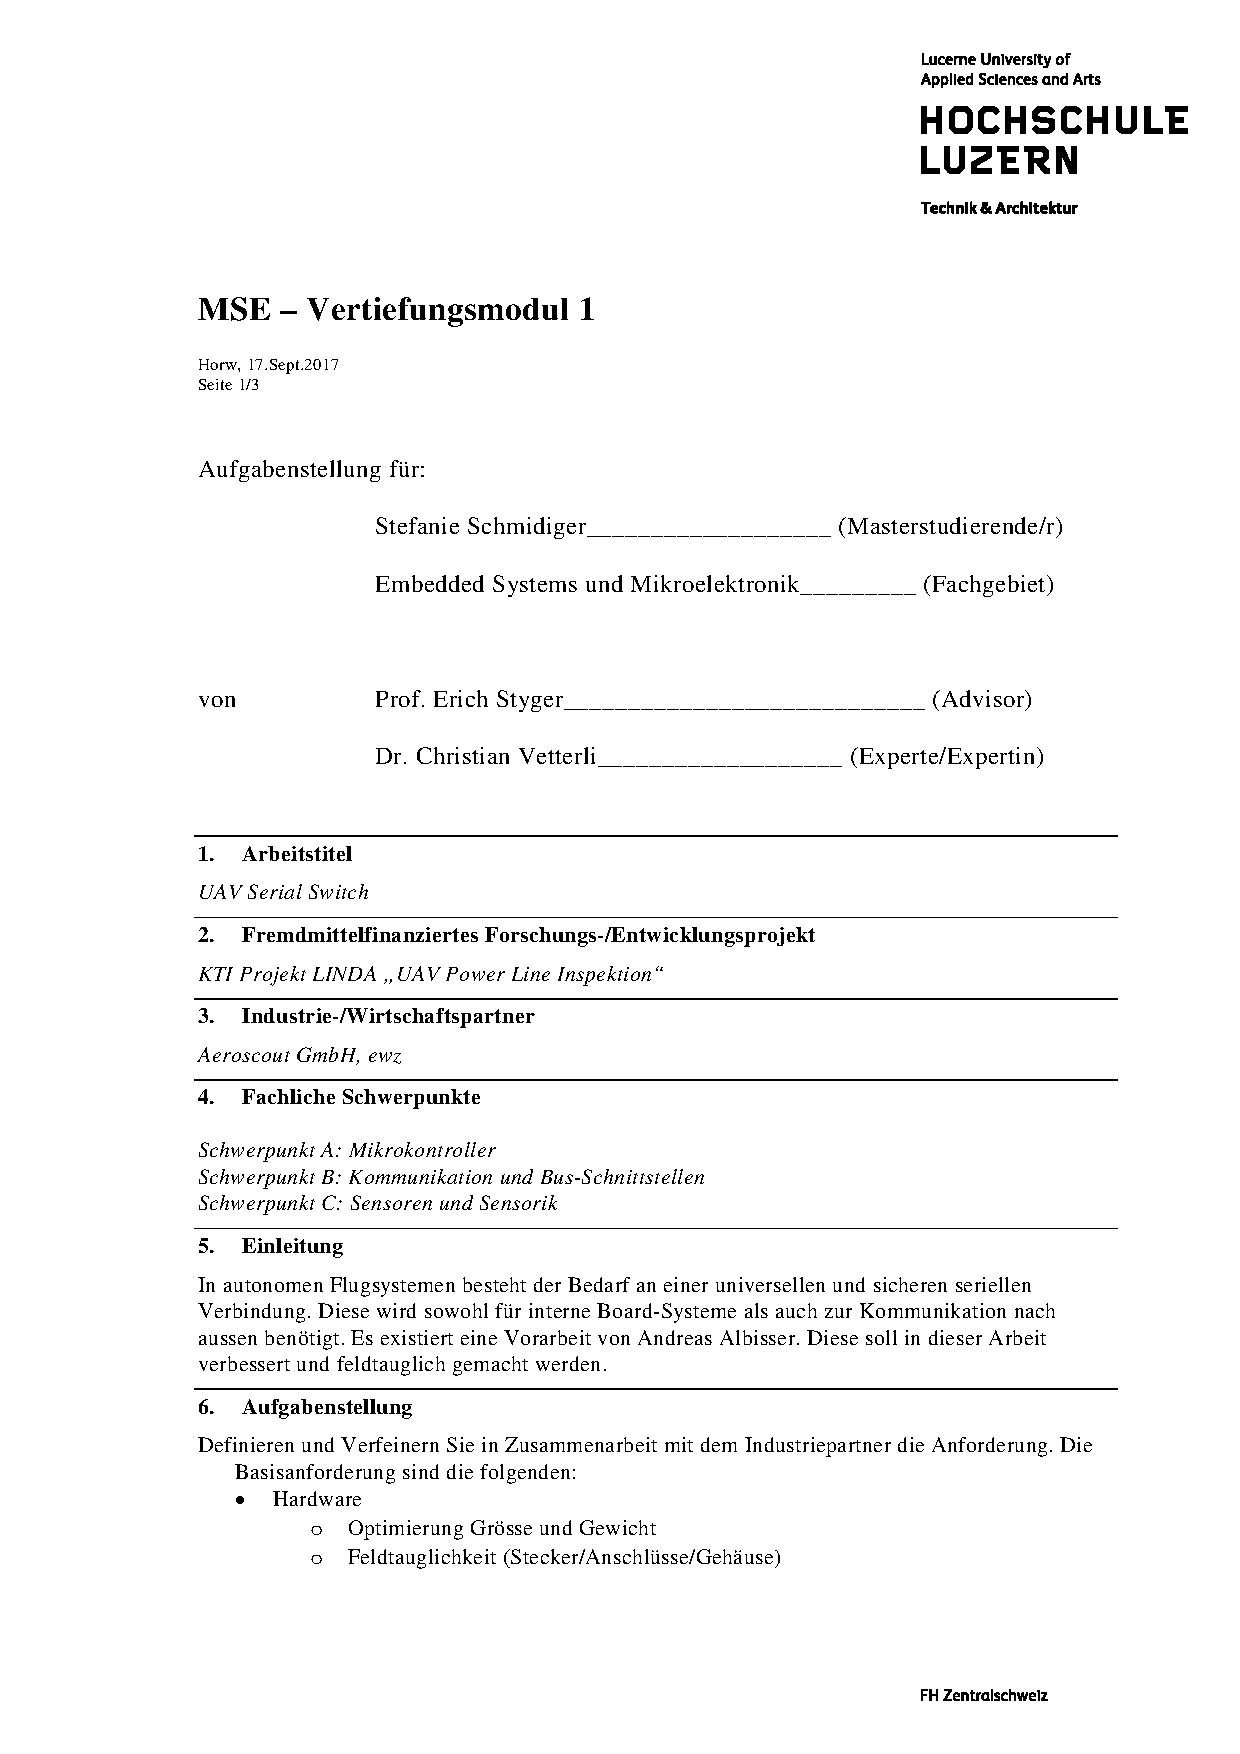
\includepdf[pages=-]{Aufgabenstellung_Vertiefungsmodul_1_Stefanie_Schmidiger.pdf}